
\documentclass[SPC-MASTER.tex]{subfiles}
\begin{document}
	\section{Pareto Chart Analysis}
{
\Large 
\begin{itemize}
\item A Pareto chart is a barplot where the categories are ordered in non increasing order, and a line is also added to show the cumulative sum.
\item Quality problems are rarely spread evenly across the different aspects of the production process or different plants. Rather, a few "bad apples" often account for the majority of problems. 
\item This principle has come to be known as the Pareto principle, which basically states that quality losses are mal-distributed in such a way that a small percentage of possible causes are responsible for the majority of the quality problems. 
\item For example, a relatively small number of "dirty" cars are probably responsible for the majority of air pollution; the majority of losses in most companies result from the failure of only one or two products. To illustrate the "bad apples", one plots the Pareto chart,
\end{itemize}
}
\newpage
\subsection{Pareto Analysis (Implementation with qcc package)}
\begin{framed}
\begin{verbatim}
defect <- c(80, 27, 66, 94, 33)

names(defect) <- c("price code", "schedule date", 
 "supplier code", "contact num.", "part num.")

# 1
pareto.chart(defect, ylab = "Error frequency")

#2
pareto.chart(defect, ylab = "Error frequency", 
    xlab = "Error causes", las=1)

#3
pareto.chart(defect, ylab = "Error frequency", 
    col=rainbow(length(defect)))

#4
pareto.chart(defect, cumperc = seq(0, 100, by = 5), 
    ylab2 = "A finer tickmarks grid")

\end{verbatim}
\end{framed}
\newpage
\textbf{Output to accompany graphs}
\begin{framed}
\begin{verbatim}
Pareto chart analysis for defect
                Frequency Cum.Freq. Percentage Cum.Percent.
  contact num.         94        94   31.33333     31.33333
  price code           80       174   26.66667     58.00000
  supplier code        66       240   22.00000     80.00000
  part num.            33       273   11.00000     91.00000
  schedule date        27       300    9.00000    100.00000
\end{verbatim}
\end{framed}
%------------------------------------------- %
\newpage

\begin{figure}[h!]
\centering
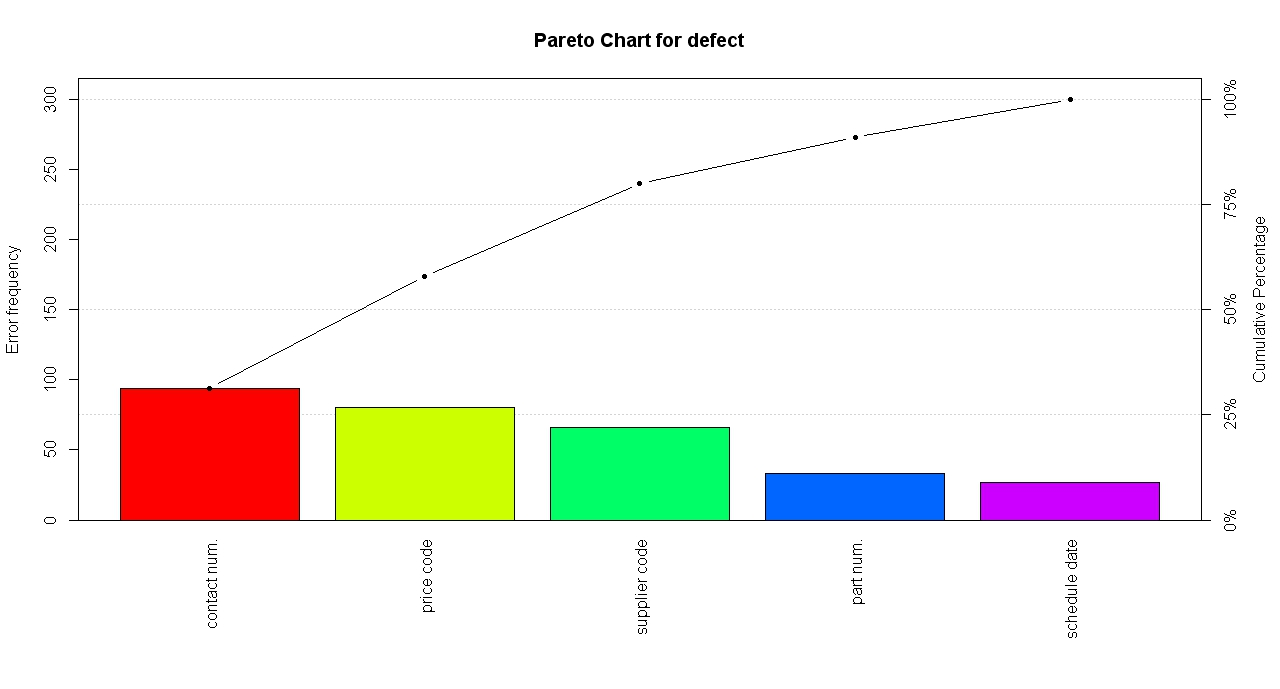
\includegraphics[width=0.9\linewidth]{images/Pareto3}
\caption{Third Implementation}
\label{fig:Pareto3}
\end{figure}

\begin{figure}[h!]
\centering
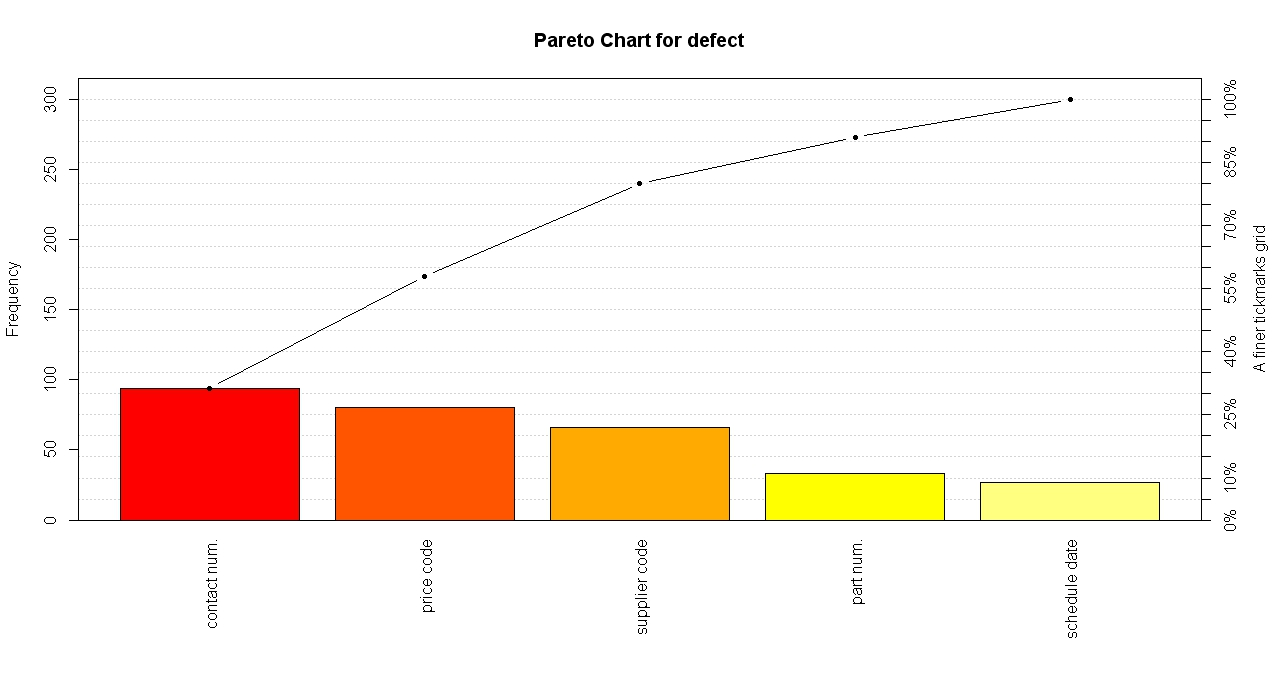
\includegraphics[width=0.9\linewidth]{images/Pareto5}
\caption{Fourth Implementation}
\label{fig:Pareto5}
\end{figure}


\subsection{Cause and Effect Diagrams}
The cause and effect diagram is also known as ``Ishikawa diagram", and has been widely used in
Quality Management. It is one of the Seven Basic Tools of Quality.
\begin{framed}
\begin{verbatim}
cause.and.effect(cause=list(
  Measurements=c("Micrometers", "Microscopes", "Inspectors"),
  Materials=c("Alloys", "Lubricants", "Suppliers"),
  Personnel=c("Shofts", "Supervisors", "Training", "Operators"),
  Environment=c("Condensation", "Moisture"),
  Methods=c("Brake", "Engager", "Angle"),
  Machines=c("Speed", "Lathes", "Bits", "Sockets")),
effect="Surface Flaws")
\end{verbatim}
\end{framed}
\begin{figure}[h!]
\centering
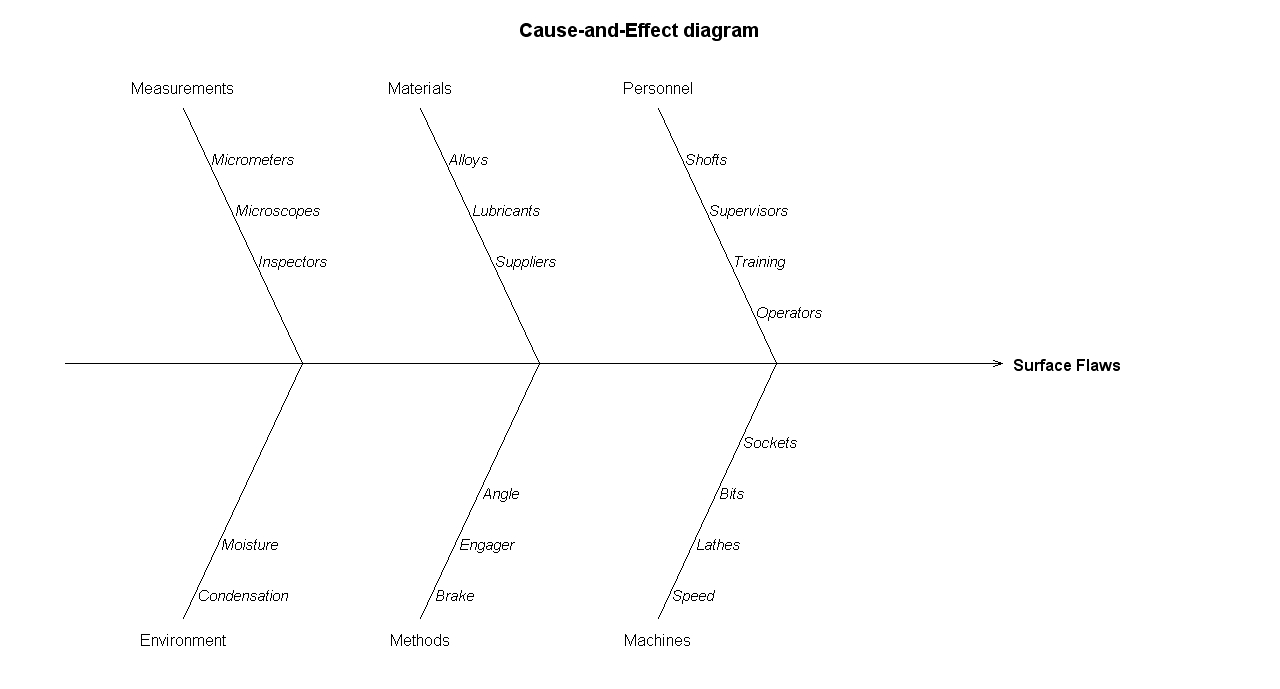
\includegraphics[width=0.7\linewidth]{./qccfishbone}
\caption{}
\label{fig:qccfishbone}
\end{figure}
\newpage
\subsubsection{Implementation with Six Sigma Package}
\begin{framed}
\begin{verbatim}
effect <- "Flight Time"
causes.gr <- c("Operator", "Environment", "Tools", "Design",
"Raw.Material", "Measure.Tool")
causes <- vector(mode = "list", length = length(causes.gr))
causes[1] <- list(c("operator #1", "operator #2", "operator #3"))
causes[2] <- list(c("height", "cleaning"))
causes[3] <- list(c("scissors", "tape"))
causes[4] <- list(c("rotor.length", "rotor.width2", "paperclip"))
causes[5] <- list(c("thickness", "marks"))
causes[6] <- list(c("calibrate", "model"))
ss.ceDiag(effect, causes.gr, causes, sub = "Paper Helicopter Project")
\end{verbatim}
\end{framed}
\begin{figure}[h!]
\centering
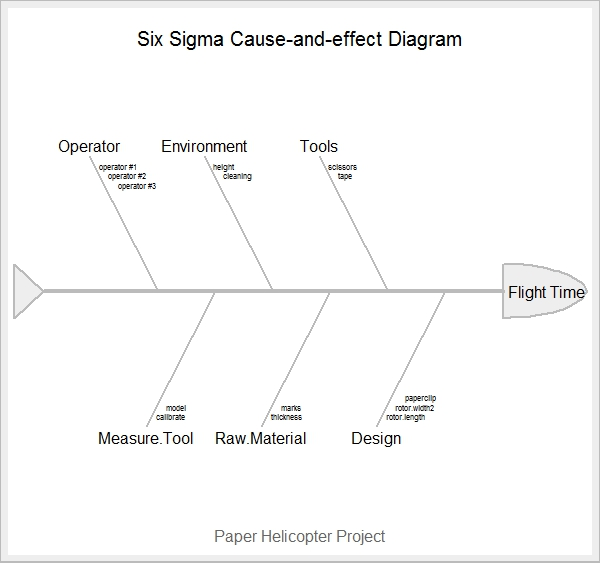
\includegraphics[width=0.7\linewidth]{./Rplot03}
\caption{}
\label{fig:Rplot03}
\end{figure}

\subsection{Constructing Process Maps}
\begin{framed}
\begin{verbatim}
inputs.overall<-c("operators", "tools", "raw material", "facilities")
outputs.overall<-c("helicopter")
steps<-c("INSPECTION", "ASSEMBLY", "TEST", "LABELING")
\end{verbatim}
\end{framed}

\begin{framed}
\begin{verbatim}
#Inputs of process "i" are inputs of process "i+1"
input.output<-vector(mode="list",length=length(steps))
input.output[1]<-list(c("sheets", "..."))
input.output[2]<-list(c("sheets"))
input.output[3]<-list(c("helicopter"))
input.output[4]<-list(c("helicopter"))
\end{verbatim}
\end{framed}
Parameters of each process
\begin{framed}
\begin{verbatim}

x.parameters<-vector(mode="list",length=length(steps))

x.parameters[1]<-list(c(list(c("width", "NC")),list(c("operator", "C")),
                        list(c("Measure pattern", "P")), list(c("discard", "P"))))
x.parameters[2]<-list(c(list(c("operator", "C")),list(c("cut", "P")),
                        list(c("fix", "P")), list(c("rotor.width", "C")),
                        list(c("rotor.length",                                                                                "C")), 
                                                             list(c("paperclip", "C")), list(c("tape", "C"))))
x.parameters[3]<-list(c(list(c("operator", "C")),
list(c("throw", "P")),
                        list(c("discard", "P")), 
                        list(c("environment", "N"))))
x.parameters[4]<-list(c(list(c("operator", "C")),
list(c("label", "P"))))
x.parameters

\end{verbatim}
\end{framed}

\begin{framed}
\begin{verbatim}
#Features of each process
y.features<-vector(mode="list",length=length(steps))
y.features[1]<-list(c(list(c("ok", "Cr"))))
y.features[2]<-list(c(list(c("weight", "Cr"))))
y.features[3]<-list(c(list(c("time", "Cr"))))
y.features[4]<-list(c(list(c("label", "Cr"))))
y.features
ss.pMap(steps, inputs.overall, outputs.overall,
        input.output, x.parameters, y.features,
        sub="Paper Helicopter Project")
\end{verbatim}
\end{framed}
\begin{figure}[h!]
\centering
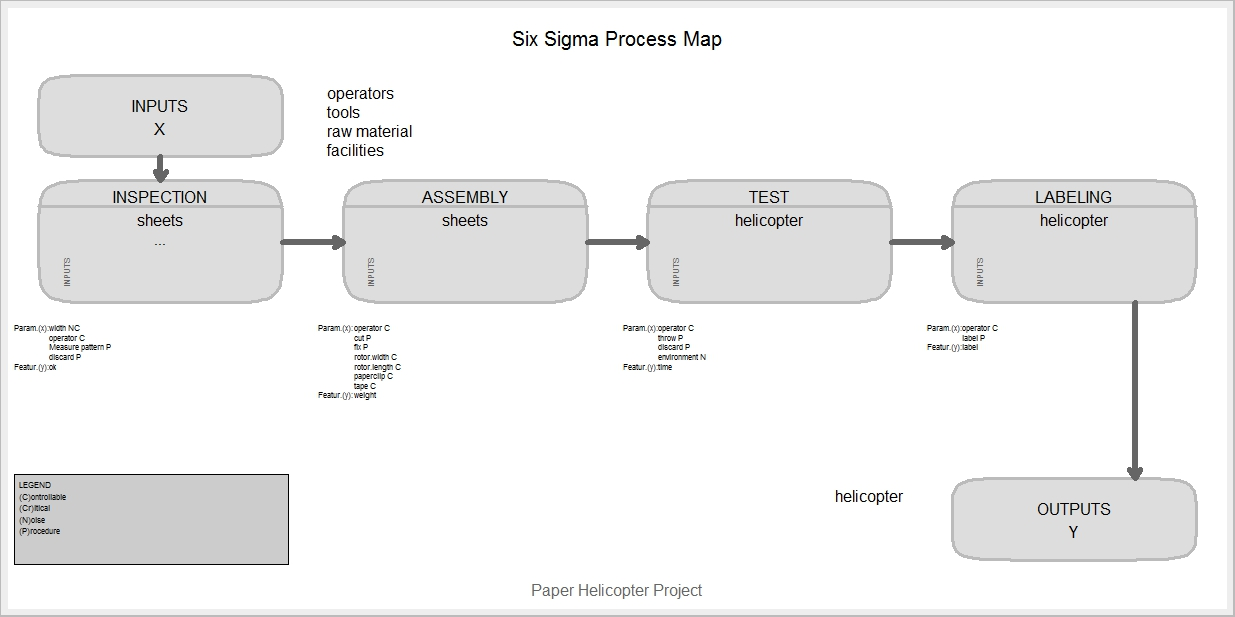
\includegraphics[width=0.9\linewidth]{./SixSigmaProcessMap}
\caption{}
\label{fig:SixSigmaProcessMap}
\end{figure}

\end{document}